\documentclass[12pt]{article}
\usepackage[utf8]{inputenc}
\usepackage{amsmath}
\usepackage{times}
\usepackage{amsfonts}
\usepackage{xcolor}
\usepackage{amssymb}
\usepackage{graphicx}
\usepackage{tabularx}
\usepackage[font=small,labelfont=bf]{caption}
\usepackage[font=small]{subcaption}
\usepackage{wrapfig}
\usepackage[section]{placeins}




\begin{document}
\vspace{20mm}

{\LARGE One-dimensional traveling waves in neuronal columns - supplemental information}

\ \\
{\bf \large Vincent Baker, vjb42@drexel.edu$^{\displaystyle 1}$}\\
{\bf \large Luis Cruz, ccruz@drexel.edu$^{\displaystyle 1}$}\\
{$^{\displaystyle 1}$Drexel University, Department of Physics.}\\

\pagebreak

\subsection*{Wave detection and labeling}
\color{red}
Our automated wave detection and labeling process must find and characterize waves under the varying conditions set by our simulation parameters.
The wave exent, wave speed, and the number of background spikes all depend upon the simulation parameters.
To validate the detection and labeling process we visually inspected the results for a variety of simulations.
Sample visualizations for varying values of $K$ are shown in Figure \ref{fig:detector_test}.
\begin{figure}[!htb]
 \caption{The clustering and wave labeling process. Spike raster plot (left), filtered clusters (middle) and labeled waves (right, each color is a unique wave) are shown for SCE with different values of $K$. }
 \label{fig:detector_test}
 \centering
   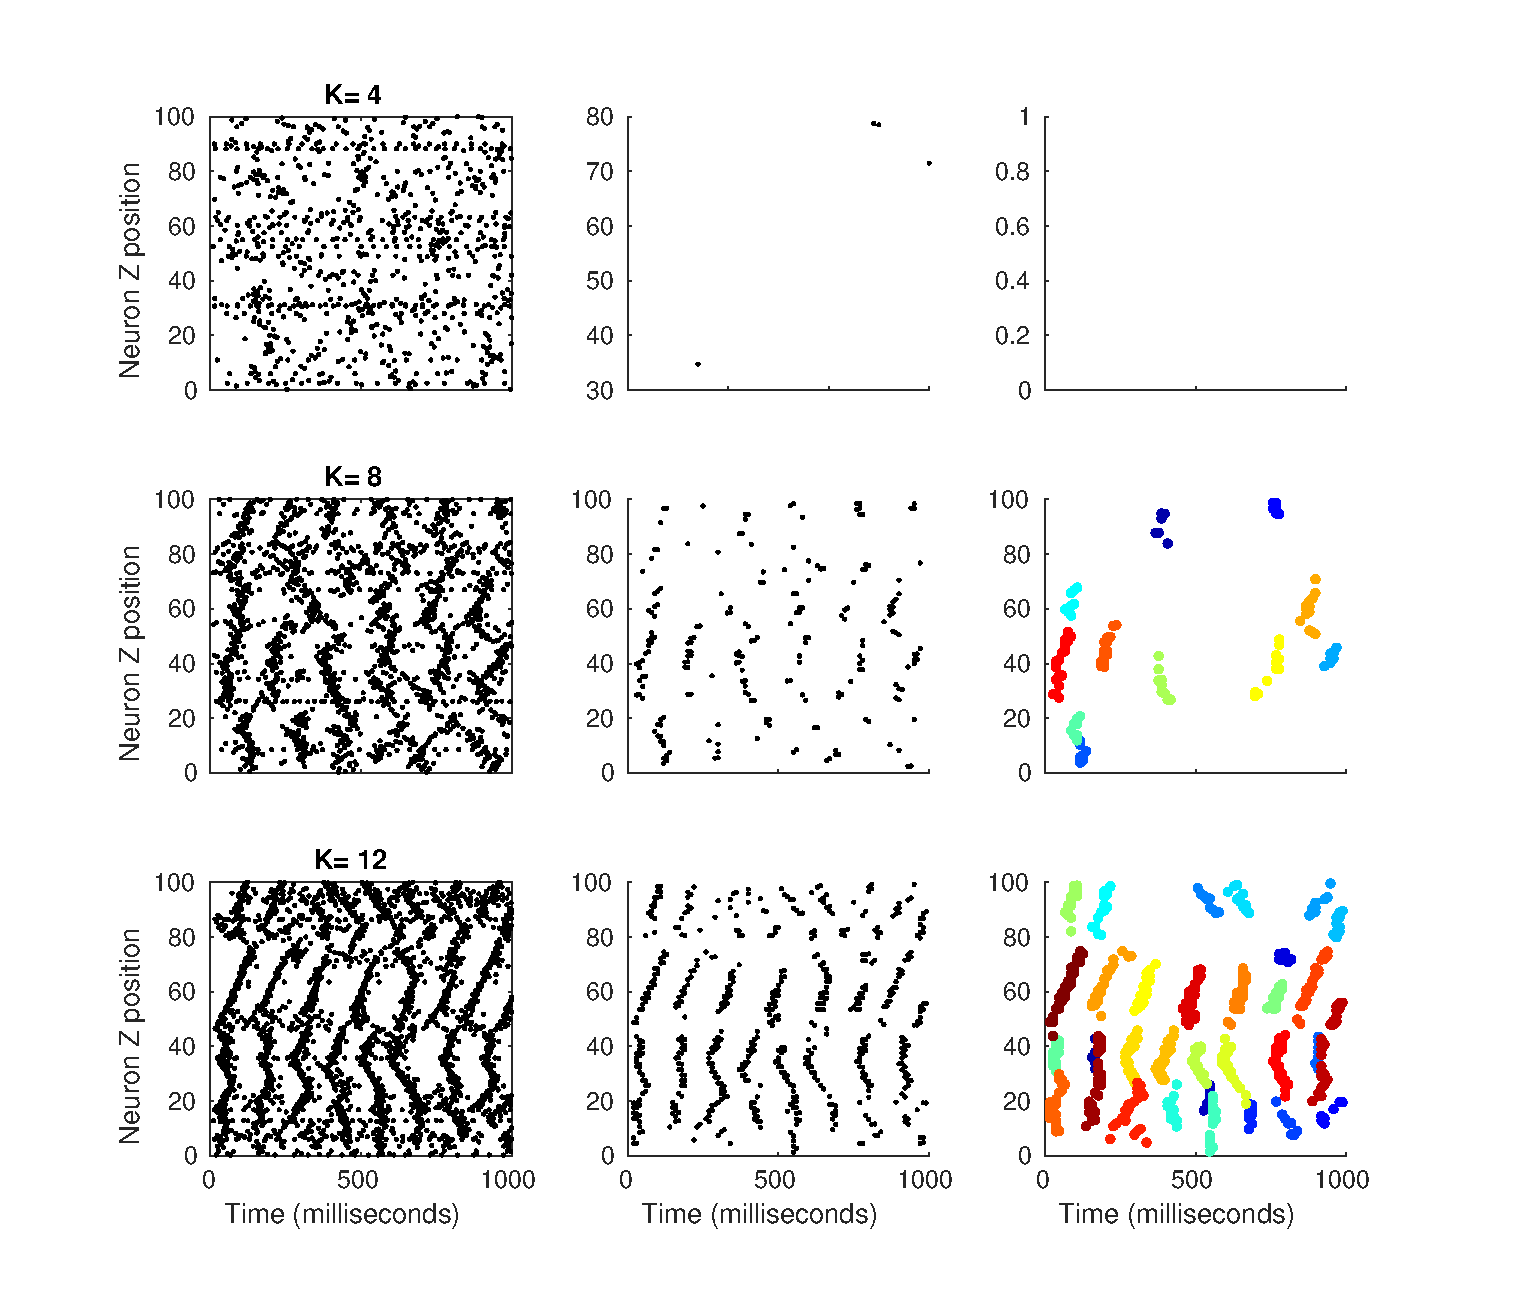
\includegraphics[width=\textwidth]{fig/DetectorTest}
\end{figure}
\FloatBarrier
\color{black}

\color{red}
\subsection*{Additional SCE statistics}
\begin{figure}[!htb]
 \caption{Distribution of (A) number of post-synaptic connections per neuron and (B) delay time. Data was taken over 100 realizations of a 2x2x50 SCE, $\lambda=2.5$, $\kappa=1$.  } 
 \begin{tabular}{c}
     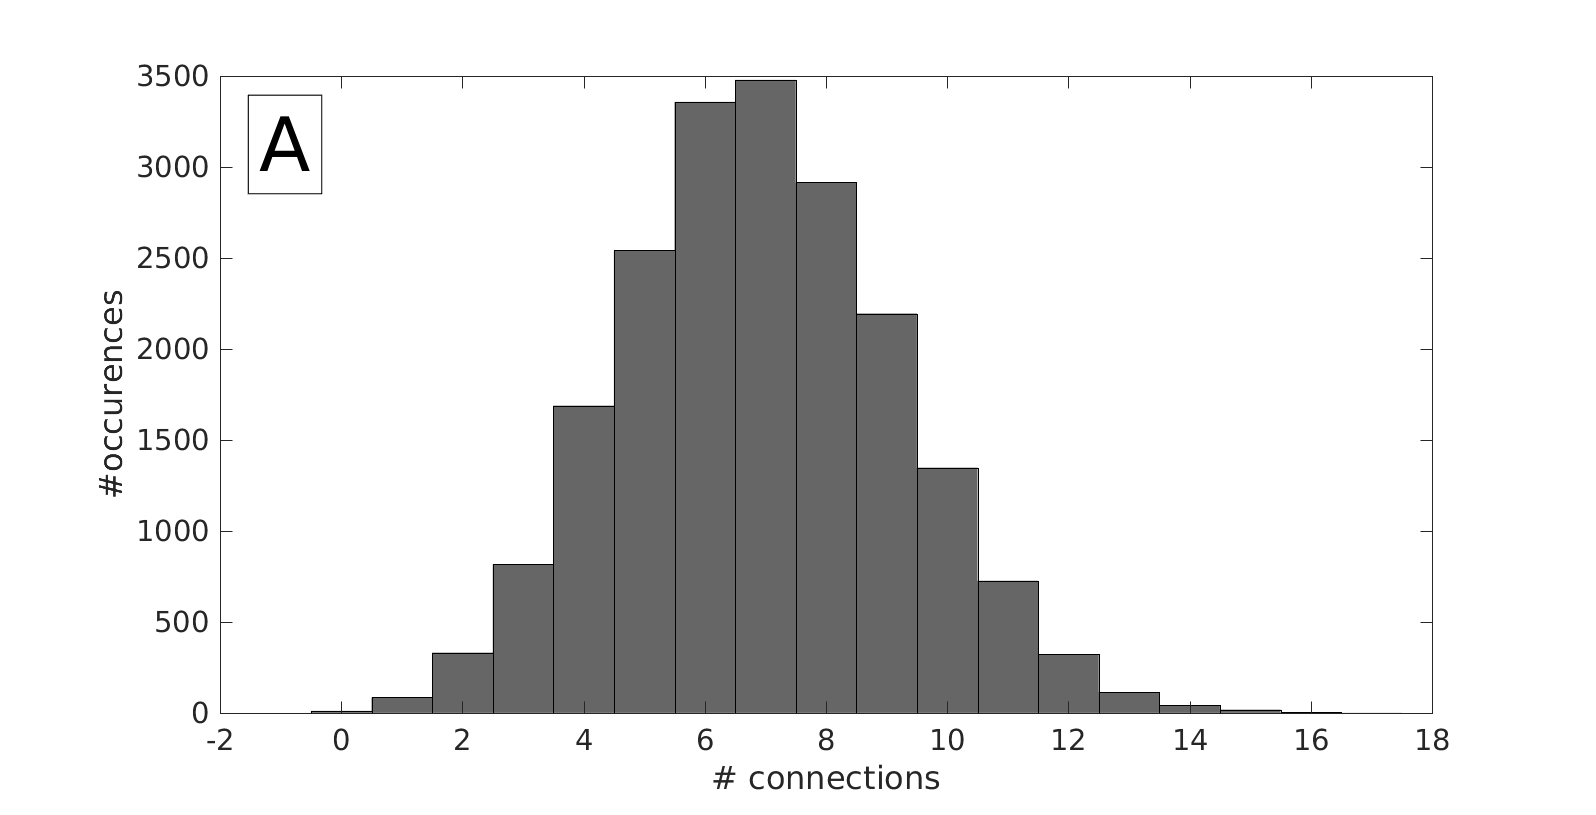
\includegraphics[width=\textwidth]{fig/ConnectionNumberDistribution} \\
     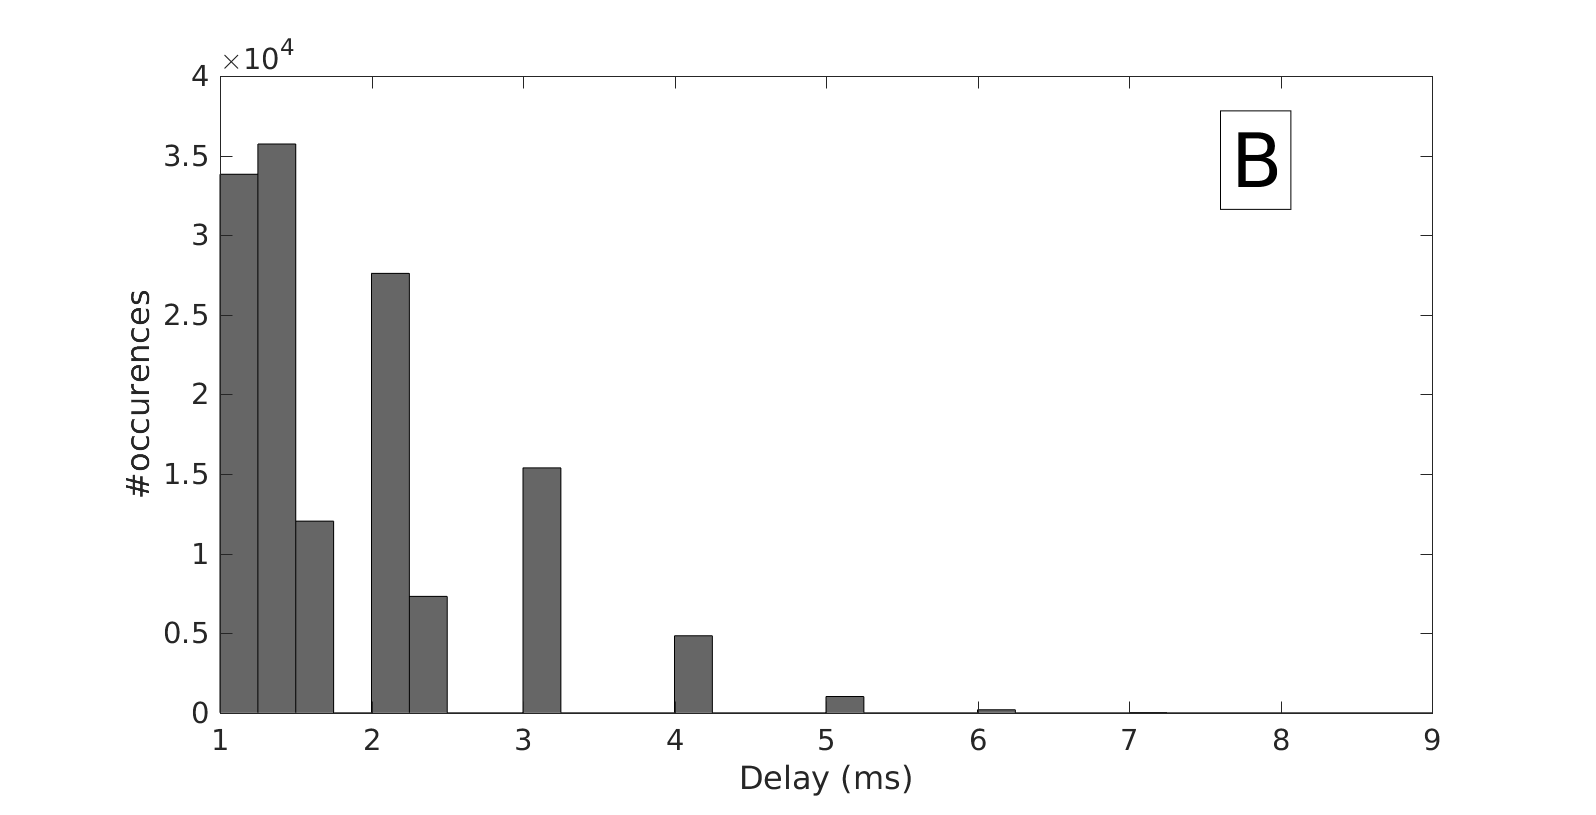
\includegraphics[width=\textwidth]{fig/DelayDistribution} 
 \end{tabular}
\end{figure}
 
\color{black}
 
\subsection*{Example FIE and FFE plots}
\begin{figure}[!htb]
 \caption{FIE and FFE for nine example columns. } 
 \begin{tabular}{ccc}
     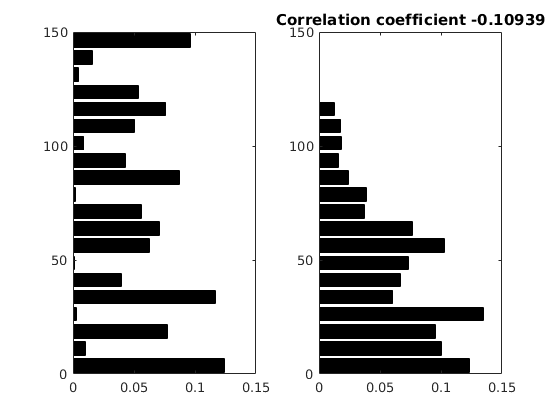
\includegraphics[width=0.3\textwidth]{fig/ccf/ccf1} & 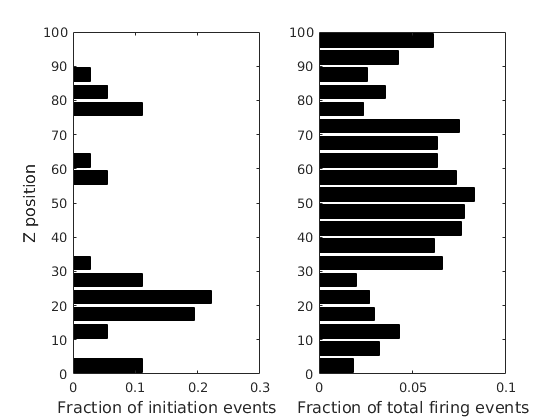
\includegraphics[width=0.3\textwidth]{fig/ccf/ccf2} & 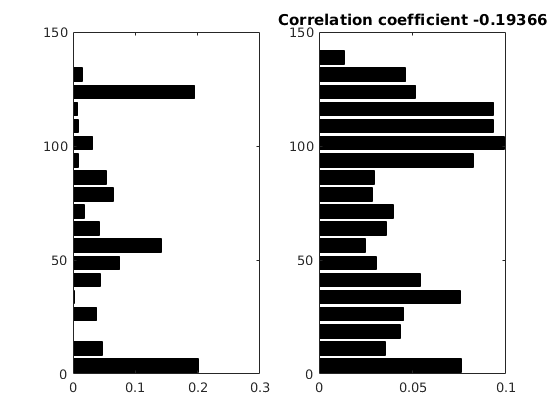
\includegraphics[width=0.3\textwidth]{fig/ccf/ccf3} \\
     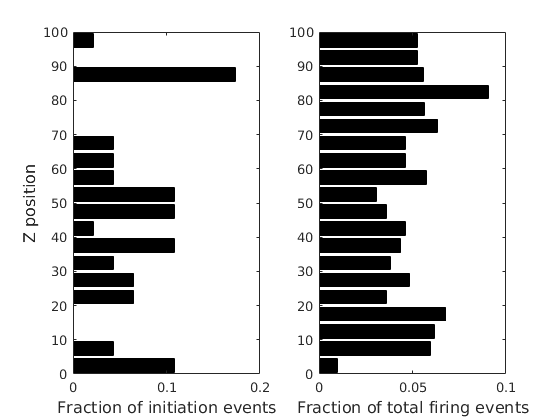
\includegraphics[width=0.3\textwidth]{fig/ccf/ccf4} & 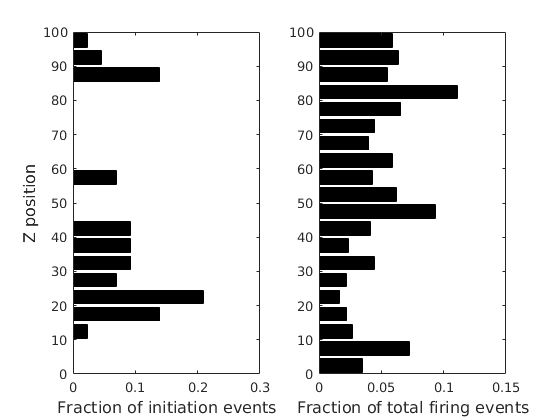
\includegraphics[width=0.3\textwidth]{fig/ccf/ccf5} & 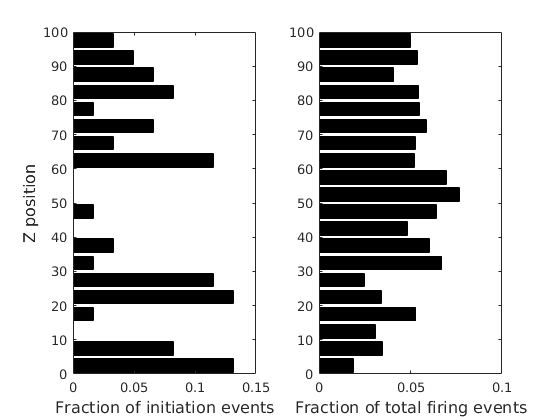
\includegraphics[width=0.3\textwidth]{fig/ccf/ccf6} \\
     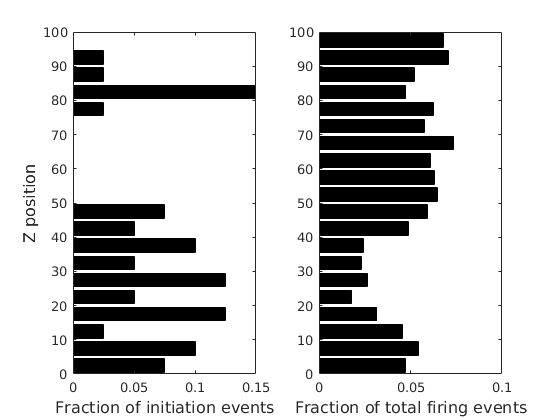
\includegraphics[width=0.3\textwidth]{fig/ccf/ccf7} & 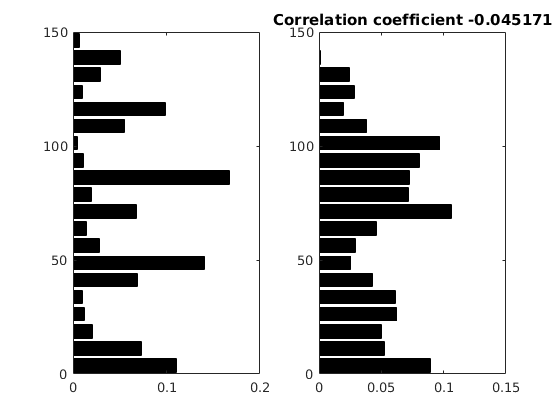
\includegraphics[width=0.3\textwidth]{fig/ccf/ccf8} & 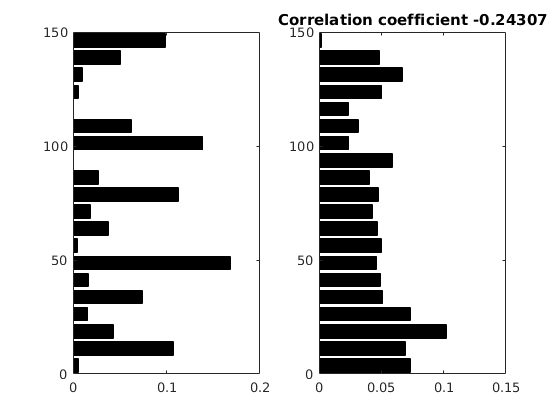
\includegraphics[width=0.3\textwidth]{fig/ccf/ccf9} 
 \end{tabular}
\end{figure}

\FloatBarrier
 
\end{document}
